\documentclass[sigplan,10pt,anonymous,review]{acmart}
\usepackage{tikz}
\usetikzlibrary{arrows.meta,positioning,calc,fit,backgrounds}
\Urlmuskip=0mu plus 2mu
\makeatletter
\g@addto@macro\UrlBreaks{\do\0\do\1\do\2\do\3\do\4\do\5\do\6\do\7\do\8\do\9%
  \do\a\do\b\do\c\do\d\do\e\do\f}
\makeatother
\setlength{\emergencystretch}{1em}
\setcopyright{none}
\settopmatter{printacmref=false,printccs=false,printfolios=true}
\acmConference[]{}{}{}
\acmBooktitle{}
\acmDOI{}
\acmISBN{}
\renewcommand\footnotetextcopyrightpermission[1]{}
\makeatletter
% Keep acmart review line numbers without the empty conference separators.
\fancypagestyle{overlapreview}{%
  \fancyhf{}%
  \renewcommand\headrulewidth{0pt}%
  \fancyhead[LE]{\ACM@linecountL}%
  \fancyhead[LO]{\ACM@linecountL\@headfootfont\shorttitle}%
  \fancyhead[RE]{\@headfootfont\@shortauthors\ACM@linecountR}%
  \fancyhead[RO]{\ACM@linecountR}%
  \fancyfoot[C]{\footnotesize\thepage}%
}
\makeatother
% Generated by paper/metrics.py. Do not edit by hand.
% Regenerate with: python3 paper/metrics.py
\newcommand{\MetricAllLeanCodeLOC}{1424}
\newcommand{\MetricAllLeanSourceLOC}{2410}
\newcommand{\MetricBoundDecimalLower}{0.38085601258978320591}
\newcommand{\MetricBoundDecimalUpper}{0.38085601258978320592}
\newcommand{\MetricBoundDenominator}{6465103708838880000000000000000}
\newcommand{\MetricBoundDenominatorBits}{103}
\newcommand{\MetricBoundFraction}{\frac{2462273619527794579322422405079}{6465103708838880000000000000000}}
\newcommand{\MetricBoundNumerator}{2462273619527794579322422405079}
\newcommand{\MetricBoundNumeratorBits}{101}
\newcommand{\MetricCarryFreeBaseThreshold}{243294782771024732160000000000000000}
\newcommand{\MetricCarryFreeBaseThresholdBits}{118}
\newcommand{\MetricCoefficientUpperBound}{25860414835355520000000000000000}
\newcommand{\MetricCoefficientUpperBoundBits}{105}
\newcommand{\MetricGainDecimalLower}{0.00000000114531579911}
\newcommand{\MetricGainDecimalUpper}{0.00000000114531579912}
\newcommand{\MetricGainDenominator}{2155034569612960000000000000000}
\newcommand{\MetricGainDenominatorBits}{101}
\newcommand{\MetricGainFraction}{\frac{2468195140225859198307}{2155034569612960000000000000000}}
\newcommand{\MetricGainNumerator}{2468195140225859198307}
\newcommand{\MetricGainNumeratorBits}{72}
\newcommand{\MetricGeneratedLeanCodeLOC}{902}
\newcommand{\MetricGeneratedLeanSourceLOC}{1802}
\newcommand{\MetricHandwrittenLeanCodeLOC}{522}
\newcommand{\MetricHandwrittenLeanSourceLOC}{608}
\newcommand{\MetricIntegerPeakBits}{102}
\newcommand{\MetricLeanTheoremDeclarations}{50}
\newcommand{\MetricPackedBaseExponent}{128}
\newcommand{\MetricPackedFixedStorageBits}{1204224}
\newcommand{\MetricPackedLeftOperandBits}{1075102}
\newcommand{\MetricPackedLeftStorageHeadroomBits}{129122}
\newcommand{\MetricPackedProductBits}{2279243}
\newcommand{\MetricPackedRightOperandBits}{1204142}
\newcommand{\MetricPackedRightStorageHeadroomBits}{82}
\newcommand{\MetricParentBoundDenominator}{323255185441944}
\newcommand{\MetricParentBoundDenominatorBits}{49}
\newcommand{\MetricParentBoundFraction}{\frac{123113681346619}{323255185441944}}
\newcommand{\MetricParentBoundNumerator}{123113681346619}
\newcommand{\MetricParentBoundNumeratorBits}{47}
\newcommand{\MetricParentCells}{4704}
\newcommand{\MetricParentSignedVertices}{9409}
\newcommand{\MetricPeakEventIndex}{7123}
\newcommand{\MetricPeakSignedVertexIndex}{7124}
\newcommand{\MetricPythonVerifierCodeLOC}{158}
\newcommand{\MetricPythonVerifierSourceLOC}{175}
\newcommand{\MetricSmallCaseCount}{8}
\newcommand{\MetricSmallCasePartitionCount}{17576}
\newcommand{\MetricWitnessCells}{9408}
\newcommand{\MetricWitnessDenominator}{52428700000000}
\newcommand{\MetricWitnessDenominatorBits}{46}
\newcommand{\MetricWitnessDistinctHeights}{5395}
\newcommand{\MetricWitnessEventCount}{18815}
\newcommand{\MetricWitnessHeightMax}{52428700000000}
\newcommand{\MetricWitnessHeightSum}{246624604800000000}
\newcommand{\MetricWitnessPeakCount}{1}
\newcommand{\MetricWitnessPeakLag}{-2284}
\newcommand{\MetricWitnessShiftDenominator}{1176}
\newcommand{\MetricWitnessShiftFraction}{-\frac{571}{1176}}
\newcommand{\MetricWitnessShiftNumerator}{-571}
\newcommand{\MetricWitnessSignedVertices}{18817}

\newcommand{\pack}{\operatorname{pack}}
\newcommand{\ct}{C_{\mathrm{cont}}}
\newcommand{\leanid}[1]{\texttt{#1}}

\begin{document}
\title[Certifying a Continuous Overlap Bound]{Certifying a Continuous Overlap Bound with One Packed Product}
\author{Anonymous Author(s)}

\begin{abstract}
A bound on an integral over every real shift can be checked through an
equality between three natural numbers. A carry-free product and a
fixed-length digit contract establish an entire list of integer
cross-correlation coefficients. Integration of pairs of equal-width
cells then identifies the overlap between grid shifts as the affine
interpolant of those coefficients. Lean~4 checks the concrete product
by kernel reduction and proves both transfer steps. For a 9,408-cell
rational profile for Erd{\H{o}}s's minimum overlap problem, the proof
gives the exact, attained continuous supremum and an upper bound on
the infimum over admissible profiles. The discrete limiting statement
takes the published convergence characterization as an explicit
premise. Checking the product theorem in a fresh Lean process with
prebuilt data took a median of 8.14 seconds across five trials,
including import, elaboration, checking and an axiom query.
\end{abstract}

\keywords{Lean 4, computational reflection, Kronecker substitution, overlap, exact certificates}
\maketitle
\pagestyle{overlapreview}

\section{The Proof Obligation}
\label{sec:problem}

Suppose a search produces a rational step function and claims that
its overlap with its complement is small at every real shift. A
checker must account for a continuum of shifts, the sign of each
shift and the validity of the candidate itself. It must also connect
the exact arithmetic used by the search to the real-valued objective.
The proof interface in this pearl makes those obligations explicit.
One integer product supplies a complete finite calculation, and a
theorem about integration determines which real functions that
calculation describes. Each half has its own preconditions and can
be applied without reference to the search.

Let $f$ be Lebesgue measurable, with $0\le f\le 1$, pointwise zero
off $[0,2)$, and $\int_{\mathbb R} f=1$. Call such a profile
\emph{admissible}. Its complement $g_f$ is $1-f$ on $[0,2)$
and zero elsewhere. Define
\begin{equation}
 \begin{aligned}
 H_f(s)&=\int_{\mathbb R} f(x)g_f(x-s)\,dx,\\
 J(f)&=\sup_{s\in\mathbb R}H_f(s).
 \end{aligned}
 \label{eq:objective}
\end{equation}
Both factors have mass one. The support convention binds the
complement to the same interval as $f$. The all-real supremum is the
ordinary supremum of the range, including its values at individual
shifts.

The concrete theorem supplies an admissible $h$ with
\begin{equation}
 \begin{aligned}
 U &= \MetricBoundFraction,\\
 J(h)&=H_h(-571/1176)=U .
 \end{aligned}
 \label{eq:U}
\end{equation}
In particular, $U<\MetricBoundDecimalUpper$. The proof of
Eq.~\eqref{eq:U} consists of an upper bound quantified over all real
$s$ and an equality at the given shift. Writing
$\ct=\inf\{J(f): f\text{ admissible}\}$ gives the separate,
unconditional conclusion $\ct\le U$. The optimum over profiles and
the optimality of $h$ remain open. The discrete limiting statement
has additional hypotheses, described in Sec.~\ref{sec:scope}.

\begin{figure}[t]
  \centering
  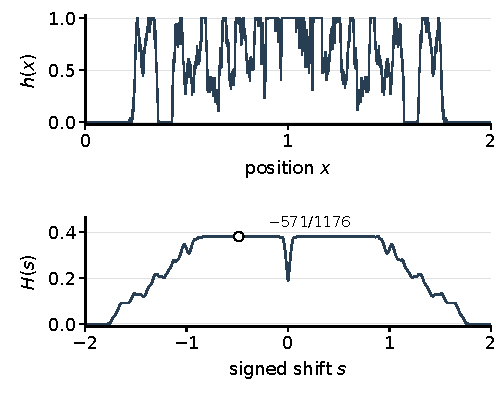
\includegraphics[width=\columnwidth]{generated/witness-profile.pdf}
  \caption{The piecewise-constant density $h$ (top) and its signed
    overlap (bottom). The polyline joins the exact grid vertices
    and has zero tails. The broad region near the maximum looks flat
    at this resolution, which cannot establish uniqueness.}
  \Description{The upper panel shows the rational step density on
    the interval from zero to two. The lower panel shows its
    continuous piecewise affine overlap with the complementary density
    as a function of signed shift, with an attaining shift marked.}
  \label{fig:witness}
\end{figure}

Figure~\ref{fig:witness} shows the witness and its overlap. The
highest region looks flat at this scale. The certificate concerns
the exact values. Its inputs are an ordered list of height
numerators, a positive denominator and a proposed coefficient
list. Its outputs include an equality of whole lists, a uniform
upper bound and, given a checked lookup, a point of attainment.
Search and file provenance can be checked using the artifact and
have no role in the logical derivation.

\section{The Integer Certificate}
\label{sec:packing}

\subsection{Encoding signed lags}

Let $a=(a_0,\dots,a_{N-1})$ with $N\ge 1$ and integer
$0\le a_i\le D$, where $D>0$. Heights are $a_i/D$ on the
cells of width $w=2/N$. The complementary height on cell $j$ is
$(D-a_j)/D$. At shift $kw$ the second cell aligns with the first
when $j+k=i$. The integer numerator of that grid value in units of
$w/D^2$ is
\begin{equation}
 T_k=\sum_{\substack{0\le i,j<N\\i-j=k}}a_i(D-a_j).
 \label{eq:lag}
\end{equation}
An empty sum is zero. The interior lags $-N<k<N$ produce
$2N-1$ coefficients. The lags $k=\pm N$ and all exterior lags
give zero.

The ordering is forced by the exponents. Write $A(z)$ for the
polynomial with coefficients $a_i$ in increasing exponent order,
and $C(z)$ for the polynomial with coefficient $(D-a_j)$ at
exponent $N-1-j$. A term $a_i(D-a_j)$ appears once in $A(z)C(z)$,
at exponent $N-1+i-j$. Consequently the product coefficient at
position $e=N-1+k$ is $T_k$. Multiplying without reversing the
complement would group pairs by $i+j$ and would compute a different
quantity. Changing the sign convention reverses the lag order.
With $g_f(x-s)$, index zero represents $k=1-N$.

Figure~\ref{fig:packing} displays the coefficient order and the
fixed-width base used for the witness.
\begin{figure*}[t]
  \centering
  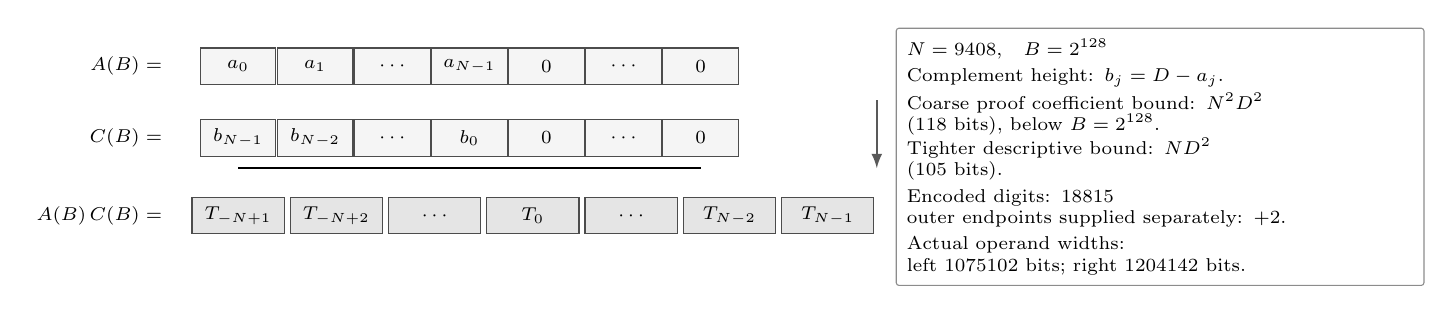
\begin{tikzpicture}[
    font=\scriptsize,
    >=latex,
    xshift=0.65cm,
    scale=0.96,
    transform shape,
    cell/.style={
      draw=black!70,
      fill=black!4,
      minimum width=1.0cm,
      minimum height=0.48cm,
      inner sep=0pt
    },
    result/.style={
      draw=black!70,
      fill=black!10,
      minimum width=1.22cm,
      minimum height=0.48cm,
      inner sep=0pt
    },
    label/.style={anchor=east, align=right},
    note/.style={
      draw=black!45,
      rounded corners=1pt,
      align=left,
      inner sep=4pt
    }
  ]
    \node[label] at (-0.88, 2.7) {$A(B)=$};
    \foreach \x/\v in {
      0/{$a_0$}, 1/{$a_1$}, 2/{$\cdots$}, 3/{$a_{N-1}$},
      4/{$0$}, 5/{$\cdots$}, 6/{$0$}
    } {
      \node[cell] at (\x*1.02, 2.7) {\v};
    }
    \node[label] at (-0.88, 1.75) {$C(B)=$};
    \foreach \x/\v in {
      0/{$b_{N-1}$}, 1/{$b_{N-2}$}, 2/{$\cdots$}, 3/{$b_0$},
      4/{$0$}, 5/{$\cdots$}, 6/{$0$}
    } {
      \node[cell] at (\x*1.02, 1.75) {\v};
    }
    \draw[thick] (0.0, 1.35) -- (6.12, 1.35);
    \node[label] at (-0.88, 0.72) {$A(B)\,C(B)=$};
    \foreach \x/\v in {
      0/{$T_{-N+1}$}, 1/{$T_{-N+2}$}, 2/{$\cdots$},
      3/{$T_0$}, 4/{$\cdots$}, 5/{$T_{N-2}$}, 6/{$T_{N-1}$}
    } {
      \node[result] at (\x*1.3, 0.72) {\v};
    }

    \node[note, text width=6.7cm, anchor=west] at (8.7, 1.5) {
      $N=\MetricWitnessCells$,\quad
      $B=2^{\MetricPackedBaseExponent}$\\[2pt]
      Complement height: $b_j=D-a_j$.\\[1pt]
      Coarse proof coefficient bound: $N^2D^2$\\
      (\MetricCarryFreeBaseThresholdBits{} bits), below $B=2^{128}$.\\[1pt]
      Tighter descriptive bound: $ND^2$\\
      (\MetricCoefficientUpperBoundBits{} bits).\\[2pt]
      Encoded digits: \MetricWitnessEventCount\\
      outer endpoints supplied separately: $+2$.\\[2pt]
      Actual operand widths:\\
      left \MetricPackedLeftOperandBits{} bits; right
      \MetricPackedRightOperandBits{} bits.
    };

    \draw[->, thick, black!65] (8.45, 2.25) -- (8.45, 1.35);
  \end{tikzpicture}
  \caption{A base-$B$ product encodes \MetricWitnessEventCount{} interior
  coefficients; lag $k$ lies at index $N-1+k$. The sufficient condition
  $B>N^2D^2$ is stronger than $B>ND^2$; the former bound has
  \MetricCarryFreeBaseThresholdBits{} bits and the latter
  \MetricCoefficientUpperBoundBits.}
  \label{fig:packing}
  \Description{A row for packed heights A and a row for reversed packed
  complements C meet at their product. The product row contains the
  18,815 interior overlap coefficients. A note states that the 118-bit
  coefficient threshold is below the 128-bit base, that the tighter
  descriptive coefficient bound is smaller, and that the actual packed
  operands have different bit widths. The 18,815 encoded entries are
  supplemented by two outer endpoints.}
\end{figure*}


For an integer base $B>1$, let $\pack_B(d)=\sum_e d_e B^e$.
The polynomial identity remains true on evaluation at $B$ for any
base, including one too small for digit recovery. The extra
arithmetic hypotheses turn that identity into the theorem used by
the checker.

\subsection{Recovering the whole list}

Let $m=2N-1$ and let $d$ be the proposed list, low order first.
The certificate establishes $|d|=m$, $0\le d_e\le P<B$, and
\begin{equation}
 \pack_B(a)\,\pack_B(\operatorname{rev}(D-a))
       =\pack_B(d).
 \label{eq:product}
\end{equation}
Here $P$ is a proposed cap in integer units. Independently of
the supplied list, the height box gives $0\le T_k$ and bounds
each summand of Eq.~\eqref{eq:lag} by $D^2$. The formal lemma
uses $T_k\le N^2D^2<B$ by bounding all pairs. Since a given
$i$ determines at most one $j$ for any fixed $k$, the elementary
bound $ND^2$ also suffices. The proof uses the looser bound
uniformly, including for lags with few contributing pairs.

By expansion the left side of Eq.~\eqref{eq:product} is the
packing of $(T_{1-N},\dots,T_{N-1})$. Long division by $B$
would recover the first digit as the remainder and the packing of
the tail as the quotient. Repeating this reasoning, and using the
known length to retain high-order zeros, identifies the entire list
with $d$. Lean uses Mathlib's fixed-length injectivity theorem for
\leanid{Nat.ofDigits}. The upper bound $T_k\le P$ follows at any
interior index without a separate dot product at that index.
The equality also transports individual lookups and is stronger
than a bound on the largest coefficient alone.

Both digit-range hypotheses matter. Equation~\eqref{eq:product}
compares integers, and division returns the carried representation
if the true coefficients are too large. An oversized proposed
digit can likewise change the list while preserving the integer.
For example $[B,0]$ and $[0,1]$ are the same length and pack to $B$.
Only the latter is a valid digit list. Even two lists with all
digits valid can pack to the same integer if their lengths differ.
A zero appended at the high end is undetectable by the equality.
The height box also controls the natural subtraction in the
complement. For $a_i>D$ the truncated difference $D-a_i$ in
\leanid{Nat} would be zero and disagree with the real complement.

\subsection{Worked example}

Take $N=3$, $D=2$, and $a=[2,1,0]$. The complement numerators are
$[0,1,2]$ and their reversal is $[2,1,0]$. Both polynomials are
$2+z$, whose product is $4+4z+z^2$. Use $B=64$, which exceeds
the formal bound $N^2D^2=36$. Both operands are $66$ and the
product $4356=4+4\cdot64+64^2$ has five required digits
$[4,4,1,0,0]$. The list $[4,4,1]$ and a six-digit list with
another high zero represent the same integer. For this input
the contract requires exactly five digits.

Those digits give, in order, the lags $-2,-1,0,1,2$. At $k=-2$
the contribution is the pair $(i,j)=(0,2)$ and equals $4$.
At $k=-1$ the pairs $(0,1),(1,2)$ contribute $2$ each.
At zero the sole nonzero term is $a_1(2-a_1)=1$.
At both positive interior lags the aligned products vanish.
The two exterior boundary vertices $k=\pm 3$ come from
support. Here $w=2/3$ and $w/D^2=1/6$. The step profile
has total mass one. The maximum is $2/3$ at both negative
vertices and on the entire interval $[-4/3,-2/3]$ joining
them, by the interpolation theorem below. The plus-shift
convention gives the reflected positive interval. Finding
one maximal digit is enough for attainment even when an
entire segment attains the same value.
The artifact's \path{scripts/PearlExample.lean} checks the exact
list and packed numerals and instantiates the affine theorem to
prove the plateau for every real parameter in the segment.

\subsection{Packing in Lean}

The concrete inputs are binary trees with natural-valued leaves.
A left subtree gives the lower powers and a right subtree is
shifted by $B$ to the power of the left size. Reversed complement
packing recurses with the right subtree in the low position and
complements at the leaves. The trees permit finite checks of size,
sum and maximum by the same decomposition. The exporter builds
balanced trees from short chunks, avoiding a linear-depth spine and
combining similarly sized packed fragments. The interface uses
only their flattened order and sizes, so correctness requires
no balancing invariant.

\leanid{Tree.pack\_eq} and \leanid{Tree.other\_eq} identify the
implementations with the two digit evaluations. A finite-sum
expansion in \leanid{packed\_events} then proves the polynomial
identity. \leanid{digits\_certified} applies the two digit
bounds and the length guard before using the equality.
This arrangement leaves list flattening and its connection to
finite sums in the reusable theory. The main product computation
takes place on the tree expressions. There are still smaller
multiplications and exponentiations in packing, reductions for
each side condition and ordinary proof checking. One packed
product refers to the multiplication of the two full operands
in Eq.~\eqref{eq:product}.

The formal expansion is a sum over finite indices. It expands
the product of the two digit evaluations and, for each pair,
inserts that term into the unique slot with the prescribed
exponent. Lean constructs this slot as an element of the
$2N-1$-element index type, justifying that it is in bounds
before summing. The insertion is represented by a sum over
all slots whose terms vanish except at that index. Exchanging
the summation order groups pairs by their slot, giving the
digit evaluation of the true list. This algebraic argument
is proved once for arbitrary inputs. At the concrete
certificate, the checker reduces a closed equality and
applies the general result without expanding its large
finite pair sum.

\section{From Grid Values to Real Shifts}
\label{sec:affine}

\subsection{Integrating a pair of cells}

The analytic theorem takes any two real-valued height vectors
$v,z$ of length $N$ and a common width $w>0$. Form the step
functions by summing constant multiples of the indicators of
$I_i=[iw,(i+1)w)$. After expanding the product at shift $s$,
the term for $(i,j)$ is $v_i z_j$ times the indicator of
$I_i\cap(I_j+s)$. The intersection is measurable and has finite
measure. Each term is integrable, so the integral distributes
over the finite sums. Its value for this pair is
$v_i z_j(R-L)_+$, where $(r)_+=\max(0,r)$ and
\[
 \begin{aligned}
 L&=\max(iw,jw+s),\\
 R&=\min((i+1)w,(j+1)w+s).
 \end{aligned}
\] This uses Lebesgue length. Endpoint
values at a finite collection of boundaries have no effect on the
integral. The Lean definitions use half-open cells throughout to
obtain pointwise cell values and pointwise zero extension.

Write $s=(k+u)w$ with $k\in\mathbb Z$ and $0\le u\le1$.
In units of $w$, translating both intervals by $-i$ gives
$[0,1)$ and $[j-i+k+u,j-i+k+u+1)$. Since $j-i+k$ is an
integer, only two positions can contribute positive length.
For $j-i+k=0$ the length in these units is $1-u$.
For $j-i+k=-1$ it is $u$. These positions are the signed
diagonals $i-j=k$ and $i-j=k+1$. When $u=0$ or $u=1$ one
of the two weights vanishes. Additional contacts at those
parameters have length zero.

Let $V_k=w\sum_{i-j=k}v_i z_j$. The two pair contributions
give the exact identity
\begin{equation}
 H((k+u)w)=(1-u)V_k+uV_{k+1}.
 \label{eq:affine}
\end{equation}
Here $H$ is the overlap of the two step functions. Choosing
$k=\lfloor s/w\rfloor$ and $u=s/w-k$ gives a valid
representation for arbitrary real $s$, including negative shifts.
Truncation toward zero would fail for negative noninteger $s/w$.
The two weights are nonnegative and sum to one, so a common bound
for the grid values applies to every real shift.

When $|k|\ge N$ the diagonal is empty and $V_k=0$. Equation
\eqref{eq:affine} implies $H(s)=0$ for $|s|\ge Nw$, with
the endpoint values also given by the grid. The finite set of
vertices from $-N$ through $N$ therefore contains a global
maximizer. Even for signed $v$ and $z$, its maximum is
nonnegative because the two endpoints are zero. The proof needs no
sign assumption on the products $v_i z_j$. What matters is the sign
of the interpolation weights and inclusion of the zero endpoints.
Tied maxima at adjacent vertices produce a maximal segment. If the
common maximum is positive and only one grid vertex attains it,
every open segment has at least one endpoint strictly below the
maximum and its interior is strictly below as well.

The finite certificate can now be used through a simple
composition rule. Extend the supplied array to a function on
integer lags by setting
\[
 \widehat d(k)=
 \begin{cases}
 d_{N-1+k}, & -N<k<N,\\
 0, & \text{otherwise}.
 \end{cases}
\]
After digit recovery, the real overlap of the rational
profile at $(k+u)w$ is
\[
 \frac{w}{D^2}\big((1-u)\widehat d(k)+u\widehat d(k+1)\big).
\]
This describes how the two formal interfaces compose.
The digit result establishes $\widehat d$ on the interior
indices. The real proof gives the scale and the exterior
indices. Interior lag bounds are needed before coercing the
signed index $N-1+k$ to a natural. For exterior lags the
proof takes the zero branch directly. This prevents natural
subtraction or truncating a negative index from silently
selecting the first digit. The dependency diagram in
Figure~\ref{fig:bridge} shows the two inputs to this
composition and the scope of the subsequent claims.

\begin{figure}[t]
  \centering
  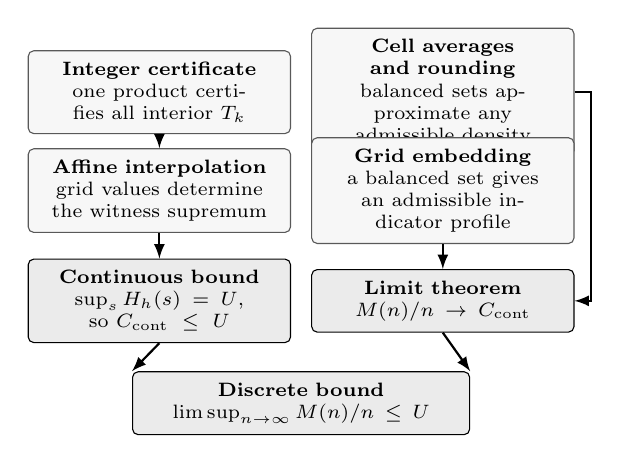
\begin{tikzpicture}[
    font=\scriptsize,
    >=latex,
    box/.style={draw=black!65, rounded corners=2pt, align=center,
      fill=black!3, text width=3.05cm, inner sep=4pt},
    claim/.style={box, draw=black, fill=black!8},
    path/.style={->, thick}
  ]
    \node[box] (digits) at (-1.80,0)
      {\textbf{Integer certificate}\\one product certifies all interior $T_k$};
    \node[box] (cells) at (1.80,0)
      {\textbf{Cell averages and rounding}\\balanced sets approximate any admissible density};
    \node[box] (affine) at (-1.80,-1.25)
      {\textbf{Affine interpolation}\\grid values determine the witness supremum};
    \node[box] (embed) at (1.80,-1.25)
      {\textbf{Grid embedding}\\a balanced set gives an admissible indicator profile};
    \node[claim] (cont) at (-1.80,-2.65)
      {\textbf{Continuous bound}\\$\sup_s H_h(s)=U$, so $\ct\le U$};
    \node[claim] (limit) at (1.80,-2.65)
      {\textbf{Limit theorem}\\$M(n)/n\to\ct$};
    \node[claim,text width=4.0cm] (disc) at (0,-3.95)
      {\textbf{Discrete bound}\\$\limsup_{n\to\infty} M(n)/n\le U$};
    \draw[path] (digits.south) -- (affine.north);
    \draw[path] (affine.south) -- (cont.north);
    \draw[path] (embed.south) -- (limit.north);
    \draw[path] (cells.east) -- ++(.21,0) |- (limit.east);
    \draw[path] (cont.south) -- (disc.north west);
    \draw[path] (limit.south) -- (disc.north east);
  \end{tikzpicture}
  \caption{The witness certifies an upper bound on the continuous infimum
  $\ct$. Rounding and grid embedding identify $\ct$ with the limit of the
  discrete minima. Both branches are formalized in Lean.}
  \label{fig:bridge}
  \Description{Two proof branches meet at the discrete bound. Packed
  coefficients and affine interpolation bound the witness supremum.
  Averaging and rounding give the upper half of the limit theorem, and
  embedding balanced sets as step functions gives the lower half.}
\end{figure}


\subsection{Instantiating the analytic theorem}
\label{sec:witness}

The file \path{construction.json} supplies the ordered numerators.
Setting the height on $I_i$ to $a_i/D$ constructs the witness.
Its parameters are
\[
 N=9{,}408,\qquad D=52{,}428{,}700{,}000{,}000,
 \qquad w=1/4704.
\]
The parent data give 4,704 numerators with denominator $524287$.
Duplicating each parent cell halves its width and leaves the parent step function pointwise unchanged
on $[0,2)$. In the witness denominator the duplicated parent
numerators are multiplied by $10^8$. Subtracting that lift from
the supplied array gives 5,396 nonzero changes, with total zero.
For example, parent cell $505$ lifts to two instances of
$11{,}900{,}000{,}000$, while witness cells $1010$ and $1011$
contain $11{,}919{,}490{,}318$ and $11{,}912{,}816{,}058$.
This describes the refinement through exact data and allows the
result to be reconstructed without the optimization history.

The new numerators satisfy the checked mass identity
\[
 \sum_i a_i=246{,}624{,}604{,}800{,}000{,}000=\frac{ND}{2}.
\] The cell integral therefore gives
$w\sum_i a_i/D=1$. The checked height box gives the pointwise
bounds on $h$ and permits the real cast of the natural
difference used for $g$. Together with measurability and support
these establish admissibility and $g=g_h$ in Lean. Substituting
$v_i=a_i/D$ and $z_j=(D-a_j)/D$ gives
$V_k=(w/D^2)T_k$ at interior vertices. The proof supplies the
exterior and boundary values separately through empty diagonals.

The embedded $18{,}815$ coefficients and the two zero endpoints
account for $18{,}817$ vertices in $[-2,2]$. The checked integer
cap is $P=4924547239055589158644844810158$, and the checked
lookup at zero-based position $7123$ gives $P$.
Since $7123=(9408-1)-2284$, the lookup corresponds to the
shift $-2284/4704=-571/1176$. Scaling the cap by
$2/(ND^2)$ gives exactly $U$. The range is nonempty, bounded
above by $U$, and contains $U$, which gives the real supremum
equality in Lean. To pass to $\ct$, admissibility supplies a
member of the objective set. Nonnegativity of the integrand for
each admissible profile gives a lower bound of zero on that set,
as required by the real infimum lemma.

\section{The Discrete Limit}
\label{sec:scope}

Let $M(n)$ minimize, over $n$-element subsets of $\{1,\dots,2n\}$,
the maximum number of ordered pairs across the partition with
difference $k$. The Lean definition uses sites in
\leanid{Fin} $(2n)$, uniformly translating the labels and
preserving signed differences. Its finite interpretation is
proved by the statement that $M(n)\le m$ holds exactly when
there exists a subset of size $n$ for which every integer
multiplicity is at most $m$. All nonzero multiplicities lie in
$-2n<k<2n$ for positive $n$.

The published characterization, due to Swinnerton-Dyer and
reported by Haugland and White, relates $M(n)/n$ to the objective
in Eq.~\eqref{eq:objective}~\cite{Haugland1996,White2023}.
Translating $[-1,1]$ by one yields the interval used here.
Changing the inclusion of the right endpoint changes each fixed
shift integral on a null set. Replacing $x+s$ by $x-s$ amounts
to reversing the shift parameter. With the zero extension the
overlap vanishes for $|s|\ge2$, so nonnegativity gives the same
supremum over all real shifts as over the published shift
interval. These convention checks are the mathematical
correspondence used to interpret the published characterization
as the premise of the Lean theorem.

\leanid{WhiteBridge} states that $M(n)/n$ tends to $\ct$.
The Lean theorem \path{discrete_upper_bound_of_white} takes
\leanid{white} of that type and a second hypothesis \leanid{hc}
that the same sequence tends to a named real $c$. Uniqueness of limits
identifies $c$ with $\ct$, and the continuous upper bound then
gives $c\le U$. The first premise carries the published
identification as well as convergence, and the second names the
limit used in the conclusion. The analytic proof of
Eq.~\eqref{eq:U} and the continuous infimum bound
require neither premise.

\section{Checking and Replaying the Certificate}
\label{sec:eval}

\subsection{Ground checks and logical dependencies}

\leanid{Numerical} imports the generated data, which import
\leanid{Tree}, whose only import is \leanid{Init}.
Seven closed facts use \leanid{decide +kernel}. They check the
height count, the height box, the height mass, the coefficient
count, the exact maximum digit, the packed product and the digit
at the attaining index. Six are axiom-free, including the
packed product. The index lookup \leanid{peak\_digit} depends on
\leanid{propext}. The generic digit transfer, real analysis and main conclusions
have the usual Lean and Mathlib dependencies
\path{propext}, \path{Classical.choice} and \path{Quot.sound}. The dependency audit reports no
\leanid{sorryAx} or project-specific axioms for these results.
Kernel reduction checks the closed equality using the embedded
literals. The external generator's evaluation of the product
is outside the Lean theorem's dependencies.

The two operands have $1{,}075{,}102$ and $1{,}204{,}142$ bits,
and their product has $2{,}279{,}243$ bits. These are actual integer
bit lengths. A fixed $128$-bit allocation for each of the $9{,}408$
positions would give $1{,}204{,}224$ bits per operand.
High-order height zeros trim the first integer, while the reversed
complement has a nonzero high digit. The formal carry bound
$N^2D^2$ has 118 bits, the elementary $ND^2$ bound has 105 bits,
and the checked peak has 102 bits. Base $2^{128}$ provides room for
both digit lists. Static counts give 522 handwritten and 902
generated Lean code lines, excluding empty and comment-only lines.
They include the library entry point and the small sample module.

\subsection{Build, replay and the isolated declaration}
\label{sec:measurements}

The artifact pins Lean~4.36.0 and locks the Mathlib revision in
\path{lake-manifest.json}. The recorded build and replay run used an
11-core Apple M3 Pro with 18 GiB of memory. It distinguishes a
project-clean default build with cached Mathlib, successive module
builds with their project predecessors already built, and
fresh-process replay against installed imports. Build commands
include driver overhead, source processing and artifact writes.
An individual module build still loads its imports. The build and
replay harness ran its commands serially. On the shared host,
background activity was neither controlled nor recorded. The
individual module bars give one elapsed time per command. The
experiment provides no distribution for repeated executions of
those commands and no elapsed-per-theorem profile.

% Generated by paper/generate_figures.py. Do not edit by hand.
% Source: benchmarks/results/20261127T033045Z/measurements.jsonl
\begin{table*}[t]
  \centering
  \caption{Selected Lean command phases from one canonical run. Each
  command contributes one wall-time and one peak-RSS observation;
  all 22 commands exited successfully.}
  \label{tab:benchmark}
  \small
  \begin{tabular*}{\textwidth}{@{\extracolsep{\fill}}lrrrr@{}}
    \hline
    Phase & Commands & Wall (s) & Max RSS (MiB) & Status \\
    \hline
    Clean & 2 & 3.840 & 673.9 & pass \\
    Module builds & 9 & 90.286 & 3560.7 & pass \\
    Default build & 1 & 29.241 & 3610.0 & pass \\
    Post-build & 1 & 1.772 & 675.3 & pass \\
    Kernel replay & 9 & 98.112 & 2804.8 & pass \\
    \hline
    Total & 22 & 223.253 & 3610.0 & pass \\
    \hline
  \end{tabular*}
  \Description{A five-row benchmark summary table. It reports
  command counts, cumulative wall time, and maximum resident memory
  for cleaning, module construction, the default build, the
  post-default benchmark build, and fresh-process kernel replay.}
\end{table*}

% Generated by paper/generate_figures.py. Do not edit by hand.
% Source: benchmarks/results/20261127T033045Z/measurements.jsonl
\begin{figure*}[t]
  \centering
  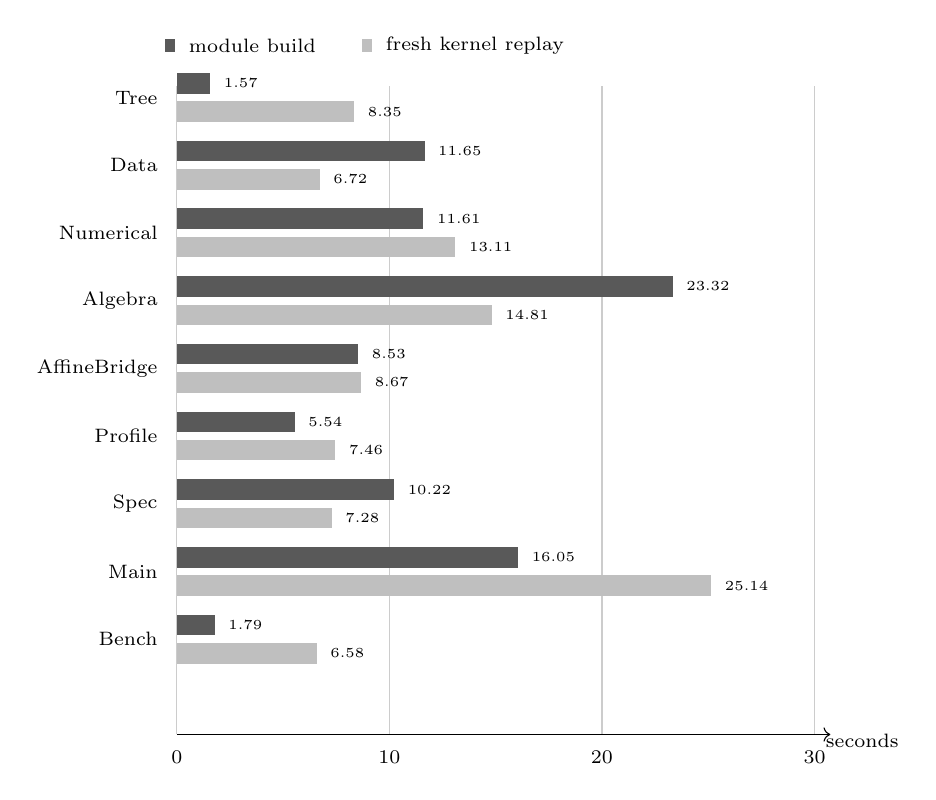
\begin{tikzpicture}[x=1cm,y=1cm,font=\scriptsize]
    \draw[black!20] (0.000,-0.350) -- (0.000,7.890);
    \node[anchor=north] at (0.000,-0.430) {0};
    \draw[black!20] (2.700,-0.350) -- (2.700,7.890);
    \node[anchor=north] at (2.700,-0.430) {10};
    \draw[black!20] (5.400,-0.350) -- (5.400,7.890);
    \node[anchor=north] at (5.400,-0.430) {20};
    \draw[black!20] (8.100,-0.350) -- (8.100,7.890);
    \node[anchor=north] at (8.100,-0.430) {30};
    \draw[->] (0,-0.350) -- (8.300,-0.350);
    \node[anchor=west] at (8.120,-0.430) {seconds};
    \fill[black!65] (-0.15,8.320) rectangle (-0.02,8.480);
    \node[anchor=west] at (0.03,8.400) {module build};
    \fill[black!25] (2.35,8.320) rectangle (2.48,8.480);
    \node[anchor=west] at (2.53,8.400) {fresh kernel replay};
    \node[anchor=east] at (-0.12,7.740) {Tree};
    \fill[black!65] (0,7.790) rectangle (0.425,8.050);
    \node[font=\tiny,anchor=west] at (0.475,7.920) {1.57};
    \fill[black!25] (0,7.430) rectangle (2.253,7.690);
    \node[font=\tiny,anchor=west] at (2.303,7.560) {8.35};
    \node[anchor=east] at (-0.12,6.880) {Data};
    \fill[black!65] (0,6.930) rectangle (3.146,7.190);
    \node[font=\tiny,anchor=west] at (3.196,7.060) {11.65};
    \fill[black!25] (0,6.570) rectangle (1.814,6.830);
    \node[font=\tiny,anchor=west] at (1.864,6.700) {6.72};
    \node[anchor=east] at (-0.12,6.020) {Numerical};
    \fill[black!65] (0,6.070) rectangle (3.133,6.330);
    \node[font=\tiny,anchor=west] at (3.183,6.200) {11.61};
    \fill[black!25] (0,5.710) rectangle (3.538,5.970);
    \node[font=\tiny,anchor=west] at (3.588,5.840) {13.11};
    \node[anchor=east] at (-0.12,5.160) {Algebra};
    \fill[black!65] (0,5.210) rectangle (6.297,5.470);
    \node[font=\tiny,anchor=west] at (6.347,5.340) {23.32};
    \fill[black!25] (0,4.850) rectangle (4.000,5.110);
    \node[font=\tiny,anchor=west] at (4.050,4.980) {14.81};
    \node[anchor=east] at (-0.12,4.300) {AffineBridge};
    \fill[black!65] (0,4.350) rectangle (2.304,4.610);
    \node[font=\tiny,anchor=west] at (2.354,4.480) {8.53};
    \fill[black!25] (0,3.990) rectangle (2.340,4.250);
    \node[font=\tiny,anchor=west] at (2.390,4.120) {8.67};
    \node[anchor=east] at (-0.12,3.440) {Profile};
    \fill[black!65] (0,3.490) rectangle (1.497,3.750);
    \node[font=\tiny,anchor=west] at (1.547,3.620) {5.54};
    \fill[black!25] (0,3.130) rectangle (2.014,3.390);
    \node[font=\tiny,anchor=west] at (2.064,3.260) {7.46};
    \node[anchor=east] at (-0.12,2.580) {Spec};
    \fill[black!65] (0,2.630) rectangle (2.759,2.890);
    \node[font=\tiny,anchor=west] at (2.809,2.760) {10.22};
    \fill[black!25] (0,2.270) rectangle (1.967,2.530);
    \node[font=\tiny,anchor=west] at (2.017,2.400) {7.28};
    \node[anchor=east] at (-0.12,1.720) {Main};
    \fill[black!65] (0,1.770) rectangle (4.334,2.030);
    \node[font=\tiny,anchor=west] at (4.384,1.900) {16.05};
    \fill[black!25] (0,1.410) rectangle (6.788,1.670);
    \node[font=\tiny,anchor=west] at (6.838,1.540) {25.14};
    \node[anchor=east] at (-0.12,0.860) {Bench};
    \fill[black!65] (0,0.910) rectangle (0.482,1.170);
    \node[font=\tiny,anchor=west] at (0.532,1.040) {1.79};
    \fill[black!25] (0,0.550) rectangle (1.776,0.810);
    \node[font=\tiny,anchor=west] at (1.826,0.680) {6.58};
  \end{tikzpicture}
  \caption{Wall times for distinct ordinary construction and
  fresh-process kernel-replay commands. Each bar is one observed
  command. The table aggregates those same commands by phase.}
  \label{fig:timing}
  \Description{A horizontal grouped bar chart. Eight rows correspond
  to the core proof modules and a ninth to the benchmark module;
  each row shows one module-build time and one fresh-process kernel
  replay time in seconds.}
\end{figure*}


The project-clean default build took 29.24 seconds and reached
3,610.0 MiB peak RSS. Fetching Mathlib and cleaning the project are
separate commands. The individual build of \leanid{Numerical}
took 11.61 seconds and reached 996.6 MiB. This module build
includes all seven checks and their imports. Figure~\ref{fig:timing}
shows the per-module timings. Table~\ref{tab:benchmark}
aggregates the phases, including the sample where listed.
Wall time is the duration of each wrapper invocation on the
parent's monotonic clock. Peak RSS is the maximum resident set size
reported by Darwin's \leanid{/usr/bin/time -l}. The reported
phase maxima are maxima across commands, while the phase wall
times are elapsed command times added together. In particular the
serialized module total and the default target build measure two
different invocations of the build system.

The eight proof modules replayed successfully in a combined
91.54 seconds, with a largest individual peak of 2,804.8 MiB.
The separately replayed sample accounts for the ninth module in
Table~\ref{tab:benchmark}. The checker loads the compiled imports
and resubmits declarations from the selected module to Lean's
kernel~\cite{MorrisonUllrichLeanchecker436}. Thus replay of
\leanid{Main} checks declarations using the imported environment.
The entire eight-module loop covers the local proof modules in
the default library's import closure, while Mathlib and Lean
imports remain installed dependencies. Build and replay share a
kernel implementation. The results measure two ways of checking
the artifact under that trust boundary.

Five further trials timed a file containing just the full packed
product theorem and its axiom query. Each trial used a fresh Lean
process with prebuilt \leanid{Overlap.Data}, outside Lake startup.
The measured unit includes parsing the file, processing the
imports, elaboration, kernel checking and the axiom query. The
median wall time was 8.14 seconds, the observed range was
4.30--8.70 seconds, and the largest product-trial peak RSS was
954.3 MiB. All five axiom queries returned an empty dependency
list. Five fresh import-only controls, run in alternating pair
order with the product trials, had median 0.49 seconds and range
0.27--0.83 seconds. The filesystem cache was left in its ordinary state. The range
captures the observed variation across whole process invocations.
The experiment gives no evidence about the cause of that variation
and does not estimate an arithmetic-only time by subtracting the
control. Both files use the same installed Lean. The raw
rows are in \path{paper/validation/product-only.jsonl}.

\subsection{Smaller exact checks}

The bundled \leanid{Overlap.Bench} sample is the 64-cell slice
starting at index $3136$ of the witness. Its 64 distinct numerators
lie strictly between $0$ and $D$, so each aligned product is
positive. In particular there are no all-zero interior
coefficients. The sample checks a packed product with 127 digits
and a separate total. Its build and replay are measured as
module commands, just as for the core. It is a test of the
arithmetic calculation on real witness data, without the
unit-mass constraint for the whole profile.

The paired slice experiment uses the first 16, 32 and 64 entries
of that same nondegenerate slice. Within each size, both versions
use the same heights, denominator, expected list and
\leanid{Overlap.Tree} import. The direct version encodes each
coefficient as a sum of products of literals, then checks
equality of the flattened lists. The packed version checks one
integer equality using the same expected coefficient tree.
Python prepares the sources and computes the expected values
before the timed commands, offline. Both proofs use
\leanid{decide +kernel}. The construction measurement includes
the wrapper, import, source elaboration, checking and writing a
compiled module. The fresh replay measurement uses the already
written module and includes the wrapper, imports and kernel
rechecking. Each cell of Table~\ref{tab:slice} is one successful
wall-time observation.

\begin{table}[t]
\centering
\caption{Matched slice checks. Each entry is elapsed seconds for a
fresh command.}
\label{tab:slice}
\begin{tabular}{@{}r rr rr@{}}
\hline
 & \multicolumn{2}{c}{Construct module} & \multicolumn{2}{c}{Replay module}\\
Cells & Direct & Packed & Direct & Packed\\
\hline
16 & 2.09 & 1.68 & 7.29 & 8.84\\
32 & 3.98 & 4.83 & 10.97 & 7.53\\
64 & 7.16 & 6.65 & 11.41 & 9.70\\
\hline
\end{tabular}
\Description{Wall times in seconds for direct and packed construction
and replay of slices of sixteen, thirty-two and sixty-four cells.}
\end{table}

The ranking changes across sizes and phases. The direct source
contains one product term per ordered pair, since each pair occurs
in exactly one sum. Both target lists contain $2n-1$ coefficients
for a slice of length $n$. The packed source uses those coefficients
and one tree for the $n$ input heights. This describes the literal
form of the supplied checks. The direct terms are unrolled into
source, so that workload includes parsing and elaborating each
expression. The
paired data control the mathematical input and target, while the
two proofs exercise different representations and reduction
paths. The direct baseline is specific to this generated source.
The experiment does not measure an optimized generic convolution,
a full-size direct verifier or an arithmetic scaling law.

\subsection{Hostile inputs and external arithmetic}
\label{sec:controls}

The artifact script \path{scripts/check_digit_guards.py} exercises
the three certificate guards with temporary Lean declarations
against the installed numerical module. All six cases gave the
expected outcomes. The original product was accepted. Changing
the least significant coefficient by one while retaining the
rest of the tree made the packed equality fail. Appending a high
zero preserved the packed integer, but the padded tree failed its
required count. The equal-length pair $[B,0]$ and $[0,1]$
preserved both count and packed value, but the uncarried list
failed the strict digit range. In each failing case, the driver
requires a failed decision on the proposition, so failure to load
an import cannot count as rejection. The controls check concrete
instances of the hypotheses used in digit recovery. They are
diagnostics rather than premises of the general argument.

The Python audit \path{audit_verify.py} evaluates the coefficients
through direct integer dot products. For $0\le k\le N$, it computes
\begin{equation*}
 \begin{aligned}
 C_k &=\sum_{i=0}^{N-1-k}a_i a_{i+k},\\
 T_{+k} &=D\sum_{i=k}^{N-1}a_i-C_k,\\
 T_{-k} &=D\sum_{i=0}^{N-1-k}a_i-C_k .
 \end{aligned}
\end{equation*}
The linear terms are suffix and prefix sums respectively. This
checks the sign ordering without unpacking the Lean product.
The audit checks the sum of all event numerators against
$(\sum_i a_i)(ND-\sum_i a_i)$. It rejects a cap one
integer unit below the reported maximum and checks exact off-grid
controls using rational interval intersections. It also independently
enumerates all $17{,}576$ labelled choices of $A$ across
$n=1,\ldots,8$ to check small discrete histograms and minima.
These enumerations exercise the finite specification. The proofs
of the real bound and the conditional limiting implication
use separate arguments.

The direct scan finds that only lag $-2284$ attains $P$.
The runner-up coefficient is
\[
 T_{-3052}=4924547239052075910263140700146.
\]
The strict finite
comparisons and Eq.~\eqref{eq:affine} together imply uniqueness
over all real shifts for this witness. The Lean theorems prove
the upper bound and the attaining equality. They use no exhaustive
strict comparison. In the plus-shift convention the attaining shift
is $+571/1176$. The packing-based \leanid{verify.py} and the
direct audit recompute the parent score from the archived parent
heights. The exact difference between that score and $U$ is
\[
 \MetricGainFraction.
\]
This exceeds $1.14531579911\times10^{-9}$. The rational
comparison and decimal enclosures are exact external arithmetic
checks. Lean states its bound directly using $U$.

\subsection{Reproducing the checks}

From the repository root, use the pinned toolchain and run
\leanid{lake exe cache get} followed by \leanid{lake build}.
For fresh replay, run \leanid{lake env leanchecker}
on each of the eight modules with names prefixed by
\leanid{Overlap.} The modules are \leanid{Tree}, \leanid{Data},
\leanid{Numerical}, \leanid{Algebra}, \leanid{AffineBridge},
\leanid{Profile}, \leanid{Spec}, and \leanid{Main}.
Run the two offline Python verifiers with assertions enabled,
as in \leanid{python3 -I -S -B audit\_verify.py}. Run the guard
script with the compiled project in place. The deterministic
exporter connects the JSON numerators and generated Lean literals
by byte-for-byte regeneration. Hashes link artifact files and
the ordered external grid output. Lean reads the literal trees
and derives its result even if these provenance checks are
performed separately.

\section{Related Work}
\label{sec:related}

Erd{\H{o}}s's minimum overlap problem asks how small the maximum overlap
over integer shifts can be when $\{1,\ldots,2n\}$ is split into two sets of
size $n$. The problem appeared in Erd{\H{o}}s's 1955 paper and is indexed
as Problem~36 in Bloom's catalogue~\cite{Erdos1955,BloomErdos36}.
Swinnerton-Dyer's theorem, proved in Haugland's account, identifies the
limit of the normalized discrete minima with a continuous infimum over
admissible densities~\cite{Haugland1996}. White states the characterization
in equation~(1.1) of the preprint and uses Fourier analysis and convex
optimization to obtain a lower bound of $0.379005$ for the limiting
constant~\cite{White2023}. Haugland later obtained an upper bound by
computing the supremum of the overlap over translations for a single
admissible step function~\cite{Haugland2016}.

AlphaEvolve used evolutionary search over programs to discover a step
function for this objective~\cite[Appendix~B.5]{Novikov2025AlphaEvolve}.
EinsteinArena made the same objective a shared optimization task, with a
public Python verifier and submissions expressed as vectors of cell
heights~\cite[\S2.3 and Appendix~A.2]{Bianchi2026EinsteinArena}. The
immediate parent of our witness is the 4,704-cell Compute Substrate
proposal dated 25 November 2026, whose record traces the construction to
EinsteinArena's Blob lineage~\cite{ComputeSubstrate2026Parent}.
From the archived integer heights~\cite{ComputeSubstrate2026ParentData},
we compute the parent's exact supremum as
\[
  \frac{123113681346619}{323255185441944}.
\]
Our 9,408-cell refinement lowers that value by more than
$1.14531579911\times 10^{-9}$. Both scores can be recomputed in exact
arithmetic from their respective integer height vectors.

The verification follows the tradition of computational reflection,
where a correctness theorem turns a computation in the logic into a
proof of a mathematical claim. Gonthier used reflection for reducibility
checks in the Coq proof of the four-color theorem, and Chaieb and Nipkow
used it for quantifier elimination in Isabelle/HOL~\cite{Gonthier2008,ChaiebNipkow2008}.
In Lean~4, the certificate's numerical predicates are discharged using
\texttt{decide +kernel}, which reduces the decision procedure in the Lean
kernel~\cite{deMouraUllrich2021,Lean436Decide}. The arithmetic uses the
standard single-evaluation form of Kronecker substitution, described by
Harvey~\cite[\S1]{Harvey2009}. We prove the packed product identity
and fixed-length certificate theorem for two nonnegative coefficient lists of
arbitrary lengths. In the overlap application, the height vector
and the reversed complementary vector pack at base $2^{128}$.
Affine interpolation then extends the certified grid values to
every real shift.

The discrete limit proof links exact-mass cell averaging to
simultaneous rounding. The endpoint selection resembles the
method of conditional expectations used to derandomize rounding
schemes~\cite{Raghavan1988}. Here coordinate-wise affinity
eliminates the first-order term in a quartic potential, and a
separate cardinality repair uses the bounded incidence of each
site at a given lag.

Xu's preliminary open-source Lean development proves convergence
of the normalized discrete minima to their liminf by a Fekete
argument and verifies several classical bounds
and finite values~\cite{Xu2026MinimumOverlap}. The convergence
theorem here identifies the discrete limit with the infimum over
admissible real densities by establishing the comparison in both
directions.

The bundled \texttt{leanchecker} tool replays each compiled module's
declarations through Lean's own kernel using the environment provided by its
imports~\cite{MorrisonUllrichLeanchecker436}. The independent
direct-sum audit checks the exact parent comparison and the
uniqueness of the witness's maximizing shift.


\section{Reuse and Limits}
\label{sec:reuse}

A new admissible rational profile on a uniform grid can use the
same proofs. It needs an ordered height array, a denominator,
a carry-free base, an equal-length proposed coefficient list,
and the closed checks for the height box, mass and packed
equality. An upper bound needs a cap on the list, whereas
equality of the supremum also needs an attaining lookup or
a proof identifying a maximizer. The witness-specific part
supplies the extent, the scale factor and the rational value
claimed for the output. The analytic theorem accepts signed
heights. The digit interface here uses natural coefficients
from heights in a box. Unequal-width cells would require
accounting for differences of individual cell boundaries in the
analytic reduction. The development applies to checking a
proposed profile. Establishing a lower bound over all admissible
profiles or formalizing the limiting characterization would
require further mathematical arguments.

\section*{Human Contributions and AI Assistance}

The human researcher selected the problem, coordinated the agents
and set the verification criteria and trusted computing base. The
criteria excluded \leanid{sorry}, \path{native_decide} and custom
global axioms. The researcher personally reviewed
\path{Overlap/Spec.lean} and \path{Overlap/Main.lean} line by line
to check the mathematical specification and the explicit
\leanid{WhiteBridge} premise, and personally ran the full local
Lean build and the separate \leanid{leanchecker} replay.

Under those constraints, GPT-6.2 Astra and GPT-6.2 Sol generated
the specific 9,408-cell witness and the Lean~4 proof scripts.
AI drafted this manuscript and assisted with experiments,
typesetting and consistency checks. Luna contributed to
benchmarking, DeepSeek to engineering, and Terra to internal
quality assurance.

\bibliographystyle{ACM-Reference-Format}
\bibliography{references}
\end{document}
